\documentclass[a4paper,12pt]{article}
\usepackage[utf8]{inputenc}
\usepackage[english]{babel}
\usepackage{amssymb,amsmath,graphicx,listings}
\usepackage{uniinput}
\usepackage[left=2cm,right=2cm,top=2cm,bottom=2cm]{geometry}
\renewcommand{\familydefault}{\sfdefault}
\newcommand{\leadingzero}[1]{\ifnum #1<10 0\the#1\else\the#1\fi}
\newcommand{\mytoday}{\leadingzero{\day}.\leadingzero{\month}.\the\year}
\newcommand{\code}[1]{\textit{#1}}
\newcommand{\unit}[1]{\ensuremath{\, \mathrm{#1}}}

\lstset{language=matlab, numbers=left,numberstyle=\footnotesize, basicstyle=\footnotesize}


\begin{document}
\title{Semester project TMA4215}
\author{10\,026 and 10\,068}
\date{\mytoday}
\maketitle
%\newpage


\section{Task}
We consider minimization problems of the type
\begin{align*}
\min_{{\bf x} \in \mathbb{R}^n} g({\bf x}),\,\, g({\bf x}):=-{\bf b}^T{\bf x} + \frac12{\bf x}^TH{\bf x}+\frac1{12}{\bf x}^TC({\bf x}){\bf x},
\end{align*}
here ${\bf b} \in \mathbb{R}^n$ and, $H$ is a $n \times n$ symmetric and positive definite matrix and $C(\bf{x})$ is a diagonal
matrix with diagonal entries $c_i x^2_i, i = 1, . . . , n$. 
Here $c_i > 0$ are the components of a vector ${\bf c} \in \mathbb{R}^n$ 
and $x_i$ are the components of $\bf{x}$. 

\section{Mathematical calculations}
At first some calculations are done.
\subsection{Positive definition of $H$}\label{definit}
Since we use only one $H$, the proof is not generally, but only for one special matrix.
Let $u=\begin{pmatrix}u_1\\u_2\end{pmatrix}\in \mathbb{R}^2\backslash \begin{pmatrix}0\\0\end{pmatrix}$, and $H= \begin{pmatrix} a&b\\b&c\end{pmatrix}$, with $a,c>0$.
\begin{align*}
{\bf u}^TH{\bf u} = au_1^2 + cu_2^2 + 2 b u_1u_2
\end{align*}
If we choose $b = \sqrt{a}\sqrt{c}$, we get
$$ = (\sqrt{a}u_1+\sqrt{c}u_2)^2 >0,$$
no matter what ${\bf u}$ is. 
$H$ is positive definite with this choice of $b$.

\subsection{Gradient}
The gradient can easily be calculated with sums.
\begin{align*}
{\bf\nabla} g 
&= {\bf \nabla}\left(-\sum_{i=1}^nb_ix_i +\frac12\sum_{i=1}^n\sum_{j=1}^n H_{ij}x_ix_j + \frac1{12}\sum_{i=1}^n c_i x_i^4\right)
\end{align*}
The two sums in the middle are divided into the diagonal element and the not diagonal elements.
All not diagonal elements are there twice, because $H$ is symmetric and therefore $H_{ij} = H_{ji}$ .
\begin{align*}
&= {\bf \nabla}\left(-\sum_{i=1}^nb_ix_i +\frac12\sum_{i=1}^n H_{ii}x_i^2 + \sum_{i=1}^n\sum_{j=1}^{i-1} H_{ij}x_ix_j + \frac1{12}\sum_{i=1}^n c_i x_i^4\right)
\\&= -{\bf b} + H{\bf x} + \frac13C{\bf x}
\end{align*}

\subsection{Hessian}
The Hessian of $g$ is easily calculable:
\begin{align*}
{\bf\nabla}^2 g =  H + C
\end{align*}

\subsection{Existence of minimum}
Let $u\in R^n$ be an arbitrary vector, except $\vec{0}$ then
$$u^T(\nabla^2g(x))u = u^T (H+C) u = u^T H u + u^TCu = u^THu + \sum_{i=1}^n c_iu_i^2x_i^2.$$
Since $H$ is positive definite, $u^THu>0$ and because $c_i>0$, $u^TCu>0$, so 
$$u^T(\nabla^2g(x))u>0$$ 
That means that the Hessian of $g$ is positive definite and therefore strictly convex and has at most one local minimum.

\subsection{Equivalence of steepest decent method and forward Euler method}


\subsection{Optimal $α$ in the steepest decent method}\label{calcalpha}
To find the optimal $α$,
$$
g\left({\bf x}^{(k+1)}\right) = g \left({\bf x}^{(k)} - α^{(k)} \nabla g({\bf x}^{(k+1)})\right)
$$
has to be minimal, so $\frac{∂}{∂α} g({\bf x}^{(k+1)})$  has to be zero.
This leads to the equation
\begin{align*}
f=&\left( {\bf b}{\bf \nabla} g - {\bf x}^T  \left(H+\frac{C}{3}\right)  {\bf \nabla}^T g\right)
 + \left( ({\bf \nabla} g) ( H + C) {\bf \nabla} g \right)α
\\+ &\left( - \sum_{i=1}^n c_i  x_i  ({\bf \nabla} g)_i^3 \right)α^2
+ \frac13\left( \sum_{i=1}^n c_i  ({\bf \nabla} g)_i^4\right)α^3 
\end{align*}
Since the function is a cubic polynomial, the limit for 
$\lim_{α\rightarrow \pm\infty}f=\pm\infty$
and because the function is continuous, there has to be at least one real zero.

The function is always rising. So only one zero is possible.


\section{Main algorithms}
\subsection{Generation of the data}
The data is generated in the function \code{data}.

\begin{lstlisting}
function [ b, H, c ] = data
	b = [ 1; 0 ];
	c = [ 200; 400 ];
	H = [ 200, 20 ; 20, 2 ];
end
\end{lstlisting}
With the calculations in chapter \ref{definit} can be easily seen that $H$ is positive definite.

\subsection{Function, gradient and Hessian of $g$}

\begin{lstlisting}
function [ g ] = g ( X )
	[ b, H, c ] = data;
	dim = size(H,1);
	C = zeros ( dim, dim );
	for i = 1 : dim
		C(i,i) = c(i) * X(i) * X(i);
	end
	g = - b' * X + 0.5 * X' * H * X + 1/12 * X' * C * X;
end
\end{lstlisting}

\begin{lstlisting}
function [ nablaG ] = grad( X )
	[ b, H, c ] = data;
	dim = size ( H, 1 );
	for i = 1 : dim
	    C(i,i) = c(i) * X(i) * X(i);
	end
	nablaG = - b + H * X + 1/3 * C * X;
end
\end{lstlisting}

\begin{lstlisting}
function [ hessG ] = hessian( X )
	[ ~, H, c ] = data;
	dim = size ( H, 1 );
	C = zeros ( dim, dim );
	for i = 1 : dim
		C(i,i) = c(i) * X(i) * X(i);
	end
	hessG = H + C;
end
\end{lstlisting}

\subsection{Minimum searching algorithm}\label{core}
All methods work similar, only line 9 has to be exchanged.
The real implementation is more complicated and is shown in the next chapter.
\begin{lstlisting}
X = [ 4; -1 ];
maxiterations = 20;
tol = 1e-8;

norm_old = norm ( grad ( X) );
condition = 1;
while condition
	maxiterations = maxiterations - 1;
	X = X - alpha * grad ( X ); % steepest decent method with constant alpha
	% X = X - optimalAlpha ( X ) * grad ( X ); % with optimal alpha
	% X = X - linsolve ( hessian ( X ), grad ( X ) ); % Newton method
	residual = norm ( grad ( X ) ) / norm_old;
	condition = (maxiterations > 0) && ( residual > tol);
end
\end{lstlisting}

\subsection{Computation of α}
For the calculation of α see chapter \ref{calcalpha}.
\begin{lstlisting}
function [ alpha_optimal ] = optimalAlpha( X )
[ b, H, c] = data;
dim = size ( H, 2 );
C = zeros ( dim, dim );
gradg = grad ( X );
a3 = 0;
a2 = 0;
for i = 1 : dim
	C(i,i) = c(i) * X(i)^2;
	a3 = a3 + c(i) / 3 * gradg(i)^4;
	a2 = a2 - c(i) * X(i) * gradg(i)^3;
end
a1 = gradg' * ( H + C ) * gradg;
a0 = b'*gradg - X' * H * gradg - 1/3 * X' * C * gradg;
alphas = roots( [ a3, a2, a1, a0 ] );
for i = 1 : 3
	if imag ( alphas ( i ) ) == 0
		alpha_optimal = alphas ( i );
	end
end
end
\end{lstlisting}
 
\section{Structure of the project}
The project can be started by executing \code{main()}. 
There the initial guess, the tolerance and the maximal number of iterations is defined. 
\code{main} first calls \code{plotmethod}, which contains a variant of the code in chapter \ref{core} and returns the relative residuals, and the points ${\bf x}^{k}$.
The change of $\bf x$ in each iteration is calculated in \code{delta} for various methods.
At the end of \code{main}, all plots are generated using the functions \code{drawfunction} and \code{drawcurve}.

To count the time a process needs, there are the functions \code{meantime}, which makes many experiments and \code{fastmethod}, which is a smaller variant of \code{plotmethod}.

\section{Results}
With the program presented above, several experiments can be done.
If not other stated, $(4,-1)^T$ is used as initial guess, $10^{-8}$ as tolerance and the number of iterations is limited to $30$.
A first look at the function with the defined values suggest the minimum is around $(0,0)^T$.
\begin{figure}[h]\label{g}
	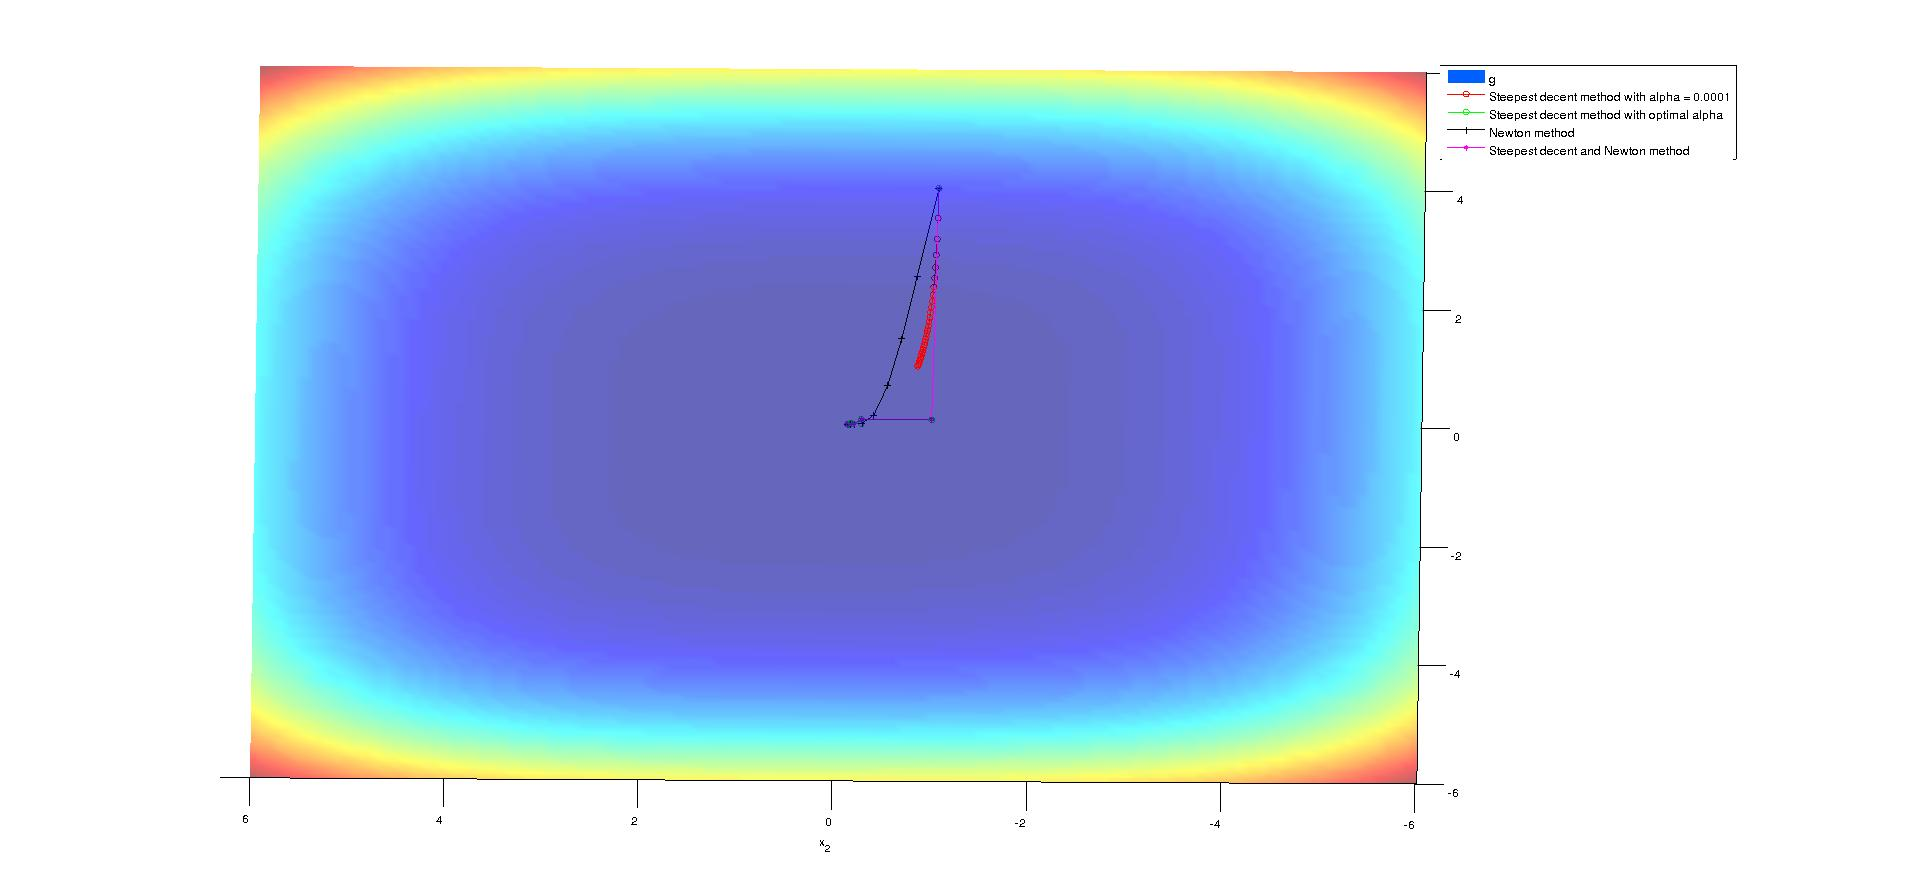
\includegraphics[width=\textwidth]{g.jpg}
	\caption{The function $g$.}
\end{figure}
\begin{figure}\label{gvalue}
	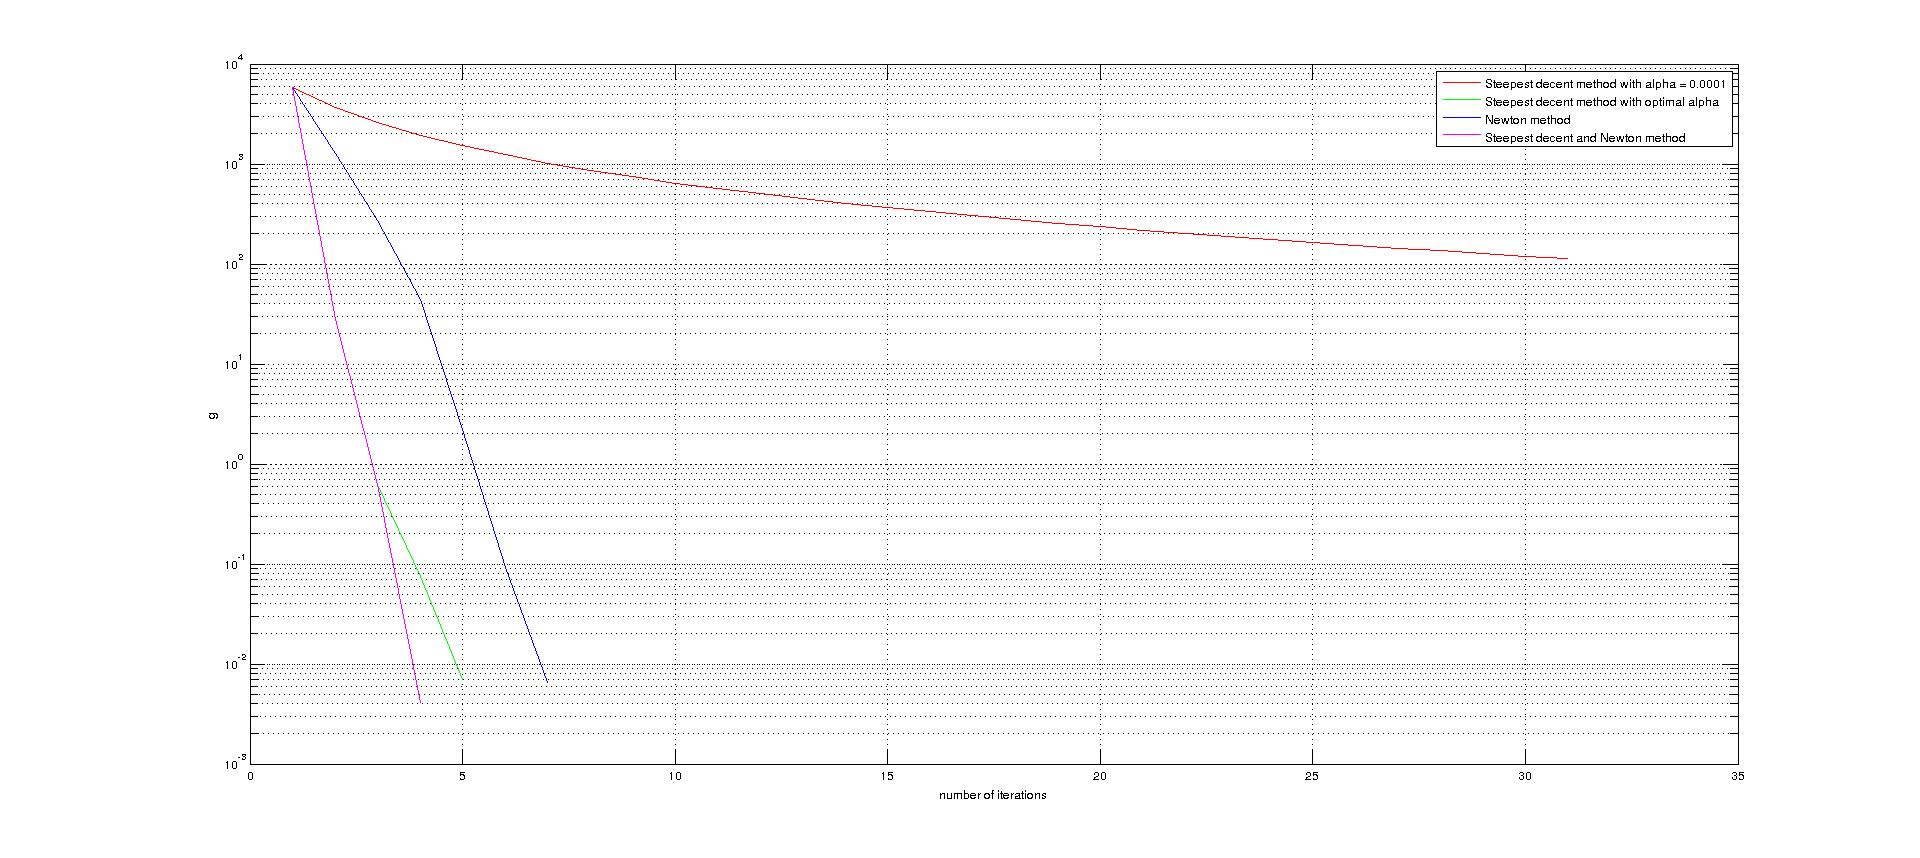
\includegraphics[width=\textwidth]{gvalues.jpg}
	\caption{The value of $g$ as a function of iterations for various methods.}
\end{figure}
\begin{figure}\label{res}
	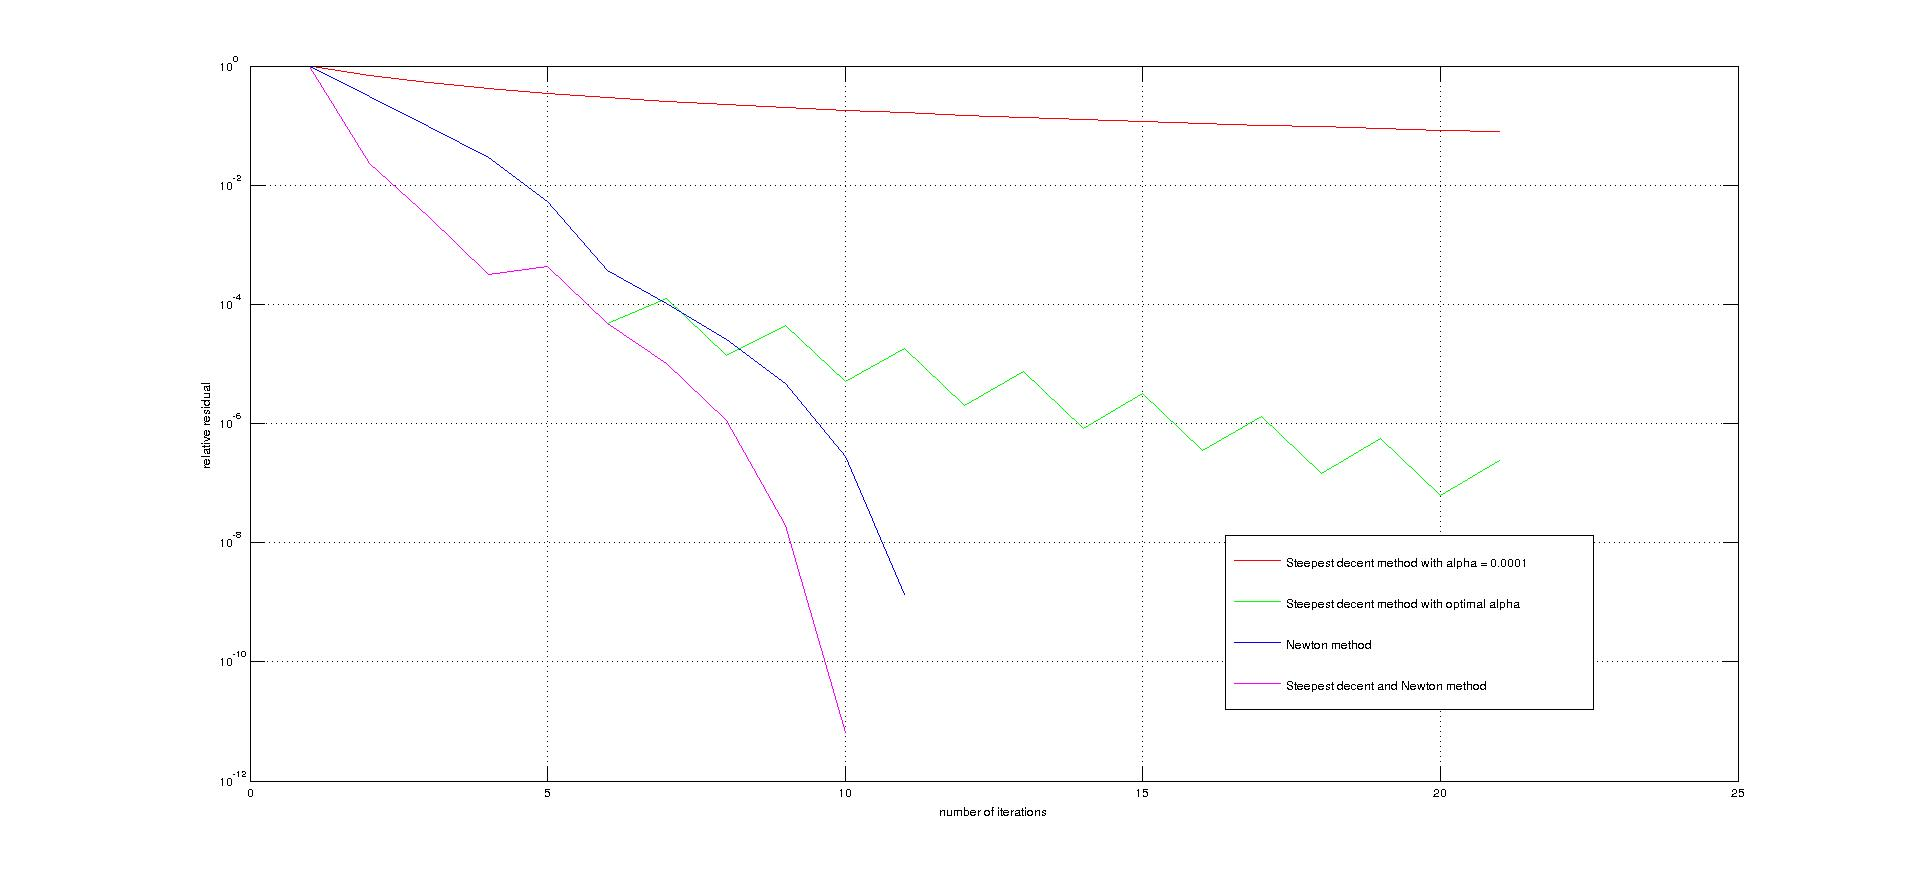
\includegraphics[width=\textwidth]{res.jpg}
	\caption{The relative residuals as a function of iterations for various methods.}
\end{figure}
\subsection{Steepest decent method with constant α}
If the initial guess is far away from the solution, the gradient at this point is very large.
To get ${\bf x}^{2}$, this gradient has to be multiplied by α.
If α is not small enough, the value of g for the next iteration gets infinity and the program breaks down.
With $α= 0.0001$, the algorithm works, but the minimum is only slowly approached.
The tolerance is reached after $744\unit{ms}$ and $25\,473$ iterations, so in most cases the limiting factor is the maximal number of iterations.

\subsection{Steepest decent method with optimal α}
The algorithm works better than with constant α, but when the relative residual drops below $10^{-3}$, the relative residual rises and falls alternately, but with a dropping drift.
It reaches the tolerance for the relative residual after 30 iterations and needs $4.33\unit{ms}$.

\subsection{Newton method}
At the beginning the Newton method reaches the minimum more slowly than the steepest  decent method with optimal α. 
After the relative residual drop below $10^{-3}$, the Newton method converges faster.
It reaches the tolerance after $1.69\unit{ms}$ and $11$ iterations.

If the initial guess for the minimum is far away from the minimum, the Newton method converges more slowly than the steepest decent method with optimal alpha.


\subsection{Steepest decent method and Newton method}
First the steepest decent method is applied and after a certain tolerance limit, the algorithm switches to the Newton method.

To find this tolerance limit, the total time for the algorithm is watched with various tolerance limits.
The program is run $1000$ times for each limit and the mean is given in tabular \ref{tab:steepestnewton}.
To run the function with minimal time, the steepest decent method is applied till the relative residual is below $10^{-2}$ and the Newton method is applied till the default tolerance ($10^{-8}$) is reached.
\begin{table}[h]
	\centering
	\label{tab:steepestnewton}
	\begin{tabular}{l||c|c|c|c|c|c}
		tolerance limit & $10^{-1}$& $10^{-2}$&  $10^{-3}$& $10^{-4}$& $10^{-5}$& $10^{-6}$\\\hline
		time $[ms]$		& 1.73&1.72&1.79&1.92&4.24&4.27
	\end{tabular}
	\caption{Times for the mixture of steepest decent and Newton method for various changing conditions.} 
\end{table}


We decided to keep the number of iterations constant, because 20 iterations is not much. 
\end{document}
